%! Author = R2D2 Team 3
%! Date = 14/04/2020

% Preamble
\documentclass[11pt]{article}
\usepackage{hyperref}
\usepackage{natbib}
\usepackage[official]{eurosym}

\usepackage{graphicx}
\usepackage{tabularx}
\usepackage{float}
\graphicspath{ {./Images/} }

\usepackage{array}

\usepackage{natbib}

\usepackage{xcolor}

\usepackage{color}
\usepackage{colortbl}

\bibliographystyle{apalike}
\renewcommand{\refname}{\section{Referenties}}

\renewcommand{\contentsname}{Inhoudsopgave}

\newenvironment{definition}
    {
        \renewcommand{\arraystretch}{1.2}
        \begin{tabular}{>{\bfseries}l >{\em}p{0.7\textwidth}}
    }
    {
        \end{tabular}
        \renewcommand{\arraystretch}{1}
    }

\newcolumntype{Y}{>{\centering\arraybackslash}X}

\newcommand{\todo}[1]{\textcolor{red}{\emph{#1}}}


\title{Gebruik van Photoplethysmography om hartslag en zuurstofsaturatie te meten in rampgebieden}

\author{\emph{R2D2 Team 3} \and Finn Fonteijn \and Youri de Vor}

% Document
\begin{document}

    \begin{titlepage}
        \centering
        \maketitle
        
\includegraphics[height=0.6\textheight]{Images/vision.jpg}
        \clearpage
    \end{titlepage}


    \clearpage
    \tableofcontents

    \clearpage

    \section{Abstract}\label{sec:abstract}
In een Rampscenario is moet de staat van elk slachtoffer gemeten worden, om zo medische zorg te geven aan degenen die het het meest nodig hebben. Twee belangrijke vitale functies, Hartslag en Zuurstofsaturatie, kunnen gemeten worden door een Pulse Oximetry sensor. Deze Research paper geeft kijkt op de theorie achter het gebruik van Photoplethysmography sensoren en vergelijkt onze hartslag implementatie van twee sensoren de MAX30100 en MAX30102, met als controle andere commerciële beschikbare sensoren. Hieruit bleek dat de MAX30102 minder variatie toonde ten opzichte van de MAX30100. Ook bleken beide sensoren een acceptabele afwijking te hebben vergeleken met onze commerciële controle producten.	
    \section{Voorwoord}\label{sec:voorwoord}
    Dit onderzoek wordt uitgevoerd in opdracht van de Hogeschool Utrecht, voor het project R2D2 2020.
    Bij dit project wordt er een ICT-bedrijf gesimuleerd.
    De werkgroep waaronder dit onderzoek valt is Team 3:\\
    \\

    \emph{
    \begin{tabularx}{\textwidth}{YYY}
        Niels Post & Otto de Visser & Amrit Malhi\\
        Menno van der Jagt & Youri de Vor & Finn Fonteijn\\
        Vincent van Setten & Oscar Kromhout
    \end{tabularx}
    \vspace{1em}
    }

    \section{Inleiding}\label{sec:inleiding}

    Het gebruik van een pulse oximeter geeft je belangrijke informatie over een aantal vitale functies van een slachtoffer. 
    Afhankelijk van de gekozen manier om deze meting uit te voeren, kan dit op een snelle, goedkope en niet-invasieve manier.
    In dit onderzoek kijken we naar verschillende meetmethoden en of deze geschikt zijn voor onze applicatie, letters B en C van de ABCDE methode voor eerste hulp. 
    Letters B en C staan voor breathing en circulation. 
    Vervolgens zullen wij kijken naar de verschillende sensoren die op de markt beschikbaar zijn, en de meest geschikte kiezen voor ons project.


    \section{Probleemstelling}\label{sec:probleemstelling}
    Voor doktoren is het lastig om een objectief pijn vast te stellen.
    Vaak moet een pati\"{e}nt zelfeen getal tussen de 1 en de 10 geven voor zijn pijn.
    Echter is deze manier van pijn inschatten niet erg objectief, daarnaast is het niet
    altijd mogelijk met de pati\"{e}nt te communiceren.
    In rampscenario's zijn er bijvoorbeeld te veel slachtoffers om aan iedereen te vragen hoeveel pijn hij voelt.
    Wel is het belangrijk om te weten hoeveel pijn mensen hebben om ze met meer/minder prioriteit te helpen.
    Hierom, in combinatie met de doelen van het R2D2 bedrijf, bestaat de vraag naar een automatische module die pijn
    detecteert.

    \section{Begrippenlijst}\label{sec:begrippenlijst}
    \paragraph{Triage}
    Triage is een middel om met beperkte capaciteit spoedzorg te organiseren. 
    In de kern betekent triage dat in een tijdsbestek van enkele minuten op basis van beperkte gegevens een beslissing genomen moet worden over hoe snel de patiënt dient te worden beoordeeld door een hulpverlener, zoals een huisarts, ambulanceverpleegkundige of een SEH-arts.    
    bron https://de-nts.nl/nts/basisprincipes-nts/

    \paragraph{PPG} 
    Photoplethysmography (PPG) is een simpele en goedkope optische meetmethode die vaak wordt gebruikt voor het controleren van hartslag doelen. 
    PPG is een niet-invasieve technologie die een lichtbron en een fotodetector op het huidoppervlak gebruikt om de volumetrische variaties in de bloedcirculatie te meten. 
    bron (https://www.ncbi.nlm.nih.gov/pmc/articles/PMC6426305/) Techniek die we gebruiken voor het meten van hartslag/zuurstof saturatie


    \paragraph{SpO2}
    Zuurstofsaturatie Perifeer,  het percentage zuurstofrijk hemoglobine (hemoglobine dat zuurstof bevat) in vergelijking met de totale hoeveelheid hemoglobine in het bloed (zuurstofrijk en niet-zuurstofrijk hemoglobine). 
    Gemeten met een externe sensor op de huid.

    \paragraph{SaO2} 
    Zuurstofsaturatie Slagaderlijk, dezelfde meeting als SpO2 maar dan verkregen via een Bloedgasmeting 


    \section{Literatuurverkenning}\label{sec:literatuur}
    \paragraph{The Feasibility of Using a Forehead Reflectance Pulse Oximeter for Automated Remote Triage(Wendelken 2004)}Het uiteindelijke doel van The Feasibility of Using a Forehead Reflectance Pulse Oximeter for Automated Remote Triage(Wendelken 2004), namelijk Remote Triage, staat heel dichtbij het doel van ons overkoepelende onderzoek. 
    Wedelken et al. kijken of het gebruik van een Reflectance Pulse Oximeter in staat is om nauwkeurig metingen van O2 Sats en Hartslag, zelfs bij signaal ruis veroorzaakt door fysieke inspanning van de proefpersoon.

    \paragraph{Mendelson 2006} heeft een portable pulse oximeter systeem ontworpen voor gebruik in Remote Triage situaties. 
    Het doel van van het systeem komt weer overeen met ons eigen onderzoek. 
    Dankzij de vooruitgangen op technologisch gebied is het ontwerp van het systeem wat verouderd, maar de uitdagingen en methodes kunnen wij nog steeds in acht nemen voor ons eigen ontwerp.

    \paragraph{Heart rate measurement based on time-lapse image} is een interessant onderzoek om te bekijken voor het bepalen van de research gap. 
    Hartslag metingen op basis van een camera zijn relevant omdat het automatisch plaatsen van sensoren voor een robot niet triviaal is. 
    In dit onderzoek is gebruik gemaakt van een toentertijd gangbare handheld camera. 
    Het type sensor van de camera is tegenwoordig niet goed meer te verkrijgen. 
    Dit heeft echter geen invloed op de relevantie van het onderzoek sinds de camera slechts werd gebruikt voor het opnemen van een time lapse. 
    De camera wordt gebruikt om een 30 seconde durende timelapse op te nemen met een interval van 200ms. 
    Het gezicht van de patiënt wordt in deze timelapse vorm opgenomen. 
    Hierna wordt voor een vakje van 3 bij 4 centimeter de gemiddelde intensiteit bepaald en hieruit wordt, na verwerking, een hartslagfrequentie uit gehaald.

    \paragraph{The non-contact monitoring of heart and respiratory rates using laser irradiation: an experimental simultaneous monitoring with and without clothes during biochemical hazards} is zeer relevant vanwege het op afstand meten van hartslag. 
    Dit wordt in dit onderzoek gesimuleerd d.m.v. konijnen. Kleding wordt gesimuleerd door middel van een klein stukje stof op de huid. 
    De metingen van deze methode zijn geverifieerd d.m.v. een ECG.

    \paragraph{Heart rate monitoring system using finger tip through Arduino and Processing Software} is een paper die gaat over het meten van hartslag op de Arduino met PPG. 
    Dit paper beschrijft zo goed als de gewenste methode van meten. 
    PPG sensoren voor de Arduino zijn een kosten effectieve en verkrijgbare hartslagmeter. 
    In de paper wordt de sensor uit losse componenten opgebouwd en wordt er gebruikt gemaakt van een Processing library.

    \paragraph{Robust Algorithm for Heart Rate (HR) Detection and Heart Rate Variability (HRV) Estimation} geeft inzage over de stappen die ondernomen moeten worden om van raw meetwaardes van een sensor naar een ecg-achtige grafiek.

    \section{Theorie en hypothese}\label{sec:theorie-en-hypothese}
    \subsection{Saturatie}
    Een te lage zuurstofsaturatie in het bloed(hypoxemie) kan leiden tot een tekort aan zuurstof toevoer aan organen of weefsel (hypoxie).
    Na enige tijd veroorzaakt dit cel dood[10], tenzij er weer zuurstof beschikbaar komt voor deze getroffen gebieden van het lichaam.

    Lage Zuurstofsaturatie in het bloed kan veroorzaakt worden door een aantal oorzaken [9], in dit onderzoek richten wij ons op oorzaken die zich voordoen na trauma of onderkoeling.
    Acute respiratory distress syndrome(ARDS) komt vaak voor na trauma of longontsteking, en is behandelbaar door reddingswerkers met zuurstof en ventilatie[8]. 
    ARDS en andere problemen met ademen/gaswisselingen in de longen zijn vaak te herkennen aan een te lage zuurstofsaturatie.

    Slagaderlijk Zuurstofsaturatie (SaO2) kan het beste gemeten worden door een Bloedgasmeting. 
    Hierbij wordt een kleine hoeveelheid bloed van een patiënt naar een klinisch-chemisch laboratorium gestuurd en wordt het bloed geanalyseerd en de meting teruggegeven. 
    [goede bron vinden] Hoewel deze methode de meest nauwkeurige resultaten terug geeft, is dit onpraktisch om een een noodsituatie  te moeten doen, en kost het kostbare tijd als een patiënt in ademnood is.

    Echter bestaat er een verband tussen en slagaderlijke zuurstofsaturatie(SaO2) en perifere zuurstofsaturatie(SpO2)[7]. 
    Dit laatste kan gemakkelijk gemeten worden door een sensor aan de buitenkant van de huid(niet invasief). 
    Er zijn bepaalde chronische /bijzondere omstandigheden waar het verschil tussen SpO2 en SaO2 van belang zijn, maar het meten van de perifere zuurstofsaturatie goed genoeg voor patiënten op de Intensive Care.[11] 
    Hierdoor zal in de rest van dit document zuurstofsaturatie altijd wijzen naar de perifere en niet de slagaderlijke zuurstofsaturatie.

    Het meten van de SpO2 wordt gedaan door middel van Photoplethysmography(PPG) Hiervoor wordt een sensor gebruikt die twee LEDs bevat, en een fotodetector. 
    Het Licht van de ene LED heeft een golflengte van 660 nm (Rood) en de andere 940 nm (InfraRood). Deze twee LEDs sturen het licht door een vinger of oor, met de fotodetector aan de weerszijde. 
    De LEDs pulseren dit omstebeurt (met pauzes er tussen om te compenseren voor omgevingslicht) ongeveer 30 keer per seconden. 
    Het geabsorbeerde licht bij deze golflengten verschilt aanzienlijk tussen bloed dat is geladen met zuurstof en bloed zonder zuurstof. 
    Zuurstofrijk hemoglobine absorbeert meer infrarood licht en laat meer rood licht door. Zuurstofarm hemoglobine laat meer infrarood licht door en absorbeert meer rood licht. 
    Vervolgens kan een microcontroller in de sensor gebruik maken van de Beer-Lambert wet om de zuurstofsaturatie uit te rekenen[12]

    Het hierboven beschreven PPG is een zogenoemde transmissive PPG, hierbij wordt het door het medium uitgezonden licht gedetecteerd door een de photodetector tegenover de LED-bron. 
    Het alternatief is een Reflective PPG, hierbij wordt het licht gedetecteerd dat terug gereflecteerd wordt door weefsel, botten en bloedvaten.

    
    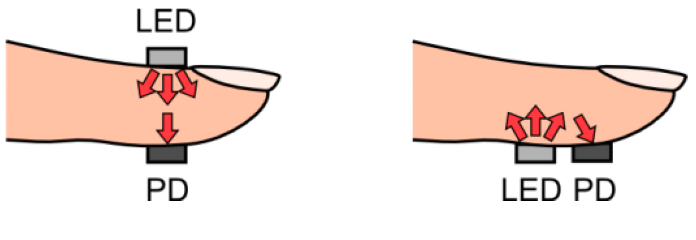
\includegraphics[height=0.2\textheight]{Images/Tamura1.png}

    \citet{tekano2007heart}

    Een transmissive PPG kan een relatief goed signaal verkrijgen, maar de meetlocatie is beperkt. 
    Om een meting te doen moet de sensor zich op het lichaam bevinden op een plaats waar doorgelaten licht gemakkelijk kan worden gedetecteerd, zoals de vingertop, het neustussenschot, de wang, de tong of de oorlel. 
    Het plaatsen van de sensor op het neustussenschot, de wang of de tong is alleen effectief onder anesthesie. 
    De vingertop en de oorlel zijn de voorkeursposities; deze plaatsen hebben echter een beperkte bloedperfusie. 
    Bovendien zijn de vingertop en de oorlel gevoeliger voor extreme omstandigheden, zoals lage omgevingstemperaturen.

    Een Reflective PPG elimineert de problemen die verband houden met de plaatsing van de sensor en er kunnen verschillende meetlocaties worden gebruikt (zoals besproken in de volgende sectie). 
    Reflective PPG wordt echter beïnvloed door bewegingsartefacten en druk storingen. 

    \subsection{Hartslag}
    Op eenzelfde manier kan de hartslag worden gemeten. 
    Volgens [Heart rate monitoring system using finger tip through Arduino and Processing Software] zetten de haarvaten in de huid van een vinger op als gevolg van een stijging in de bloeddruk tijdens een hartslag. 
    Deze verandering in formaat kan worden gemeten d.m.v. PPG.

    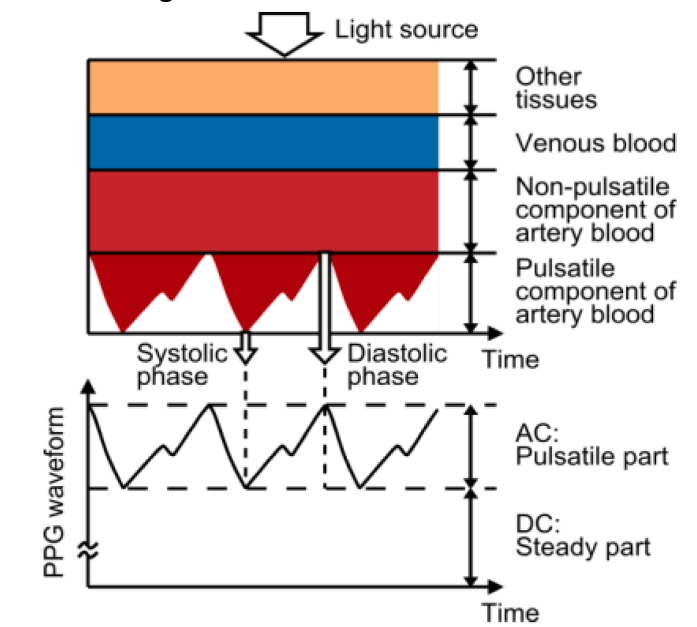
\includegraphics[height=0.5\textheight]{Images/Tamura2.png}

    
    Hartslag is een minstens zo belangrijke metriek als zuurstofsaturatie. Het is algemeen bekend dat zowel een te lage, te hoge als een onregelmatige hartslag kunnen negatieve gevolgen hebben voor de gezondheid. 
    Ook kan er op deze manier vastgesteld worden of de patiënt überhaupt een hartslag heeft.
    Daarnaast is het vaststellen van een hartaanval ook mogelijk door het meten van de onderlinge tussenposes. 

    Te hoge hartslag kan een indicatie zijn van onder andere bloedverlies, koorts, infectie, gebrek. 
    Deze oorzaken zijn veelvoorkomend tijdens rampsituaties aangezien lichamelijke letsel een veel voorkomend gevolg is van een rampsituatie. 
    De gevolgen van een te hoge hartslag zijn kortademigheid, duizeligheid, flauwvallen, zwakte en moeheid.
    [Symptoom Snelle regelmatige hartslag (tachycardie) - Symptomenchecker]

    Te lage hartslag is ook een belangrijke metriek. 
    Dit kan onder andere dienen als indicatie van onderkoeling, bloedingen en een verhoogde hersendruk, naast andere oorzaken. 
    Een te lage hartslag kan leiden tot duizeligheid, kortademigheid, vermoeidheid, hartkloppingen, flauwvallen, en geheugenstoornissen. 
    [Bradycardie (te lage hartslag) - hoe herken je het?WELKE BRON IS DIT YOURI]

	\section{Hypothese}\label{sec:hypothese}

Wij verwachten dat een reflectieve sensor is waarschijnlijk beter geschikt voor onze gestelde use case. Reflectieve sensoren kunnen op de huid worden gedrukt en dus met relatief minimale moeite door de robot geplaatst worden om zo een meting te doen. Relatief minimaal verwijst naar het monteren van een transmissieve sensor op iemand die bewusteloos is. Voor deze sensor moet een vinger of teen door de robot gevonden worden om de sensor te monteren. Dit is in verhouding significant minder triviaal dan het duwen van de sensor op een arm of been. 

Het gebruik van een specifieke sensor voor Hartslag en Pulse Oximetry vereist minder implementatie en waarschijnlijk is dit daarom de betere optie over een sensor zoals de TRCT5000. Dit is in essentie ook een reflectieve emitter met light activated transistor, maar deze moet zelf ingesteld worden met weerstanden om parameters aan te passen zoals de stroom die door de LED loopt. Ook zouden er 2 van deze sensoren moeten worden gebruikt omdat een enkele TRCT5000 alleen maar 1 golflengte licht uitstraalt, en voor het meten van Zuurstof saturatie moet er gebruik gemaakt worden van twee verschillende golflengtes.



\section{Methode}\label{sec:methode}
Dit onderzoek begint met een literatuuronderzoek naar eerder gebruikten methoden voor het meten van hartslag en zuurstofsaturatie. Er zal worden bekeken of deze eventueel geschikt zijn. Daarnaast zal er naar sensoren gezocht worden die goed verkrijgbaar zijn en ingezet kunnen worden voor de gestelde doeleinden.

\subsection{Gekozen Sensoren}
HIER IETS OVER MAX 102 100 WAT VERSCHIL IS EN WAROM WE HEBBEN GEKOZEN

\subsection{Gebruik van de Sensor}\label{subsec:gebruik van de sensor}
Beide sensoren zijn geïmplementeerd door middel van C++. Dit wordt gedaan door middel van de hwlib. Een in C++ geschreven software library ontworpen voor het zo dicht mogelijk op de hardware programmeren. De communicatie met de Arduino gaat via een i2c bus. Hiervoor is een wrapper geschreven om de bij het project bijgeleverde i2c bus gebruiksvriendelijker te maken. Alle gebruikte code is te vinden op https://gitlab.com/r2d2-2020/modules/health_monitor/-/tree/feature-max3010x

\paragraph{tests} De werking van de research code zal worden getest. Dit zal worden gedaan door middel van unit tests. Hieronder vallen tests of de sensor succesvol aangesloten is en deze i2c communicatie accepteert. Dit wordt getest door naar de interne registers van de sensor te schrijven en deze vervolgens uit te lezen. Ook zal er worden getest of de waarden die worden gemeten realistisch zijn(b.v. Revision ID is gelijk of  kleiner dan de meest recent revision van de sensor, of dat bepaalde config registers veranderd kunnen worden)


Vergelijken met andere Sensoren

Het vergelijken van de sensoren wordt door COVID-19 bemoeilijkt. Om de implementatie spoedig te laten verlopen is de hardware onder de onderzoekers verspreid. De sensoren kunnen dus niet op dezelfde persoon getest worden. In plaats hiervan zullen de sensoren worden vergeleken met andere hartslagmeters in het bezit van de onderzoekers.

MAX30100
- Samsung Galaxy S8+ ingebouwde hartslagmeter
- Xiaomi Mi Band 2

MAX30102
- Sport Horloge Met Optische Sensor(Amazfit Bip)
- Niet Optische hartslagband ( POLAR H10)
- Losse Pulse Oximeter


FOTO HIER ZETTEN
FOTO HIER ZETTEN
FOTO HIER ZETTEN

/subsection{SpO2 Metingen}

De MAX sensoren zullen helaas niet kunnen worden geïmplementeerd als SpO2 meters. Voor het meten van deze waarden is, naar wat wij gevonden hebben. Een fourier transformatie en verdere verwerking nodig. Dit is goed mogelijk, maar de Arduino Due heeft niet veel rekenkracht. Er zou ook gebruik kunnen worden gemaakt van Autocorrelatie[72] voor hartslag en SpO2. Of dit computationeel goedkoper is moet blijken uit verder onderzoek. 


[72] Piotrowski, Z., & Różanowski, K. (2010). Robust algorithm for heart rate (HR) detection and heart rate variability (HRV) estimation. Acta Physica Polonica A, 118(1), 131-135.


\subsection{Testmethode voor max30102}
Elke Proefpersoon heeft na enkele minuten rust op een stoel, alle 4 de sensoren aangesloten gekregen, en is er om de 30 seconden een meting gedaan. Na elke meting wordt de bpm die elke sensor aangeeft vastgelegd.

Sommige Metingen zijn geschrapt uit het onderzoek omdat een van de sensoren een abnormale(meer dan het dubbele van andere sensoren of 0) meting weergeeft. Opmerkenswaardig is dat alle sensoren af en toe een slechte meting gaven, en dat ook de commerciële producten vatbaar waren voor ruis of slechte meettechniek.

De controle Sensoren bestaan uit: Polar H10 Hartslagband(op basis van elektrocardiografie), Losse Pulse Oximeter Sensor (Transmissive PPG), Een Amazfit Bip Watch(Reflective PPG 530 nm), MAX30102(Reflective PPG 660 nm)

De tabel hieronder laat het absolute procentueel verschil van elke meting van de MAX30102 ten opzichte van het gemiddelde van de 3 controle metingen.

 -percentage Var =Abs((((Polar + Bip+ Losse)/3)-MAX30102)/MAX30102)

Vervolgens zijn er 5 tot 10 Metingen gedaan per Proefpersoon
Elk van de Controle sensoren is ook vergeleken met de andere twee controle sensoren voor referentie om de nauwkeurigheid commerciële sensoren te tonen.


\subsection{Testmethode voor max30100}

Elke Proefpersoon heeft na enkele minuten rust op een stoel, alle 3 de sensoren aangesloten gekregen, en is er om de 30 seconden een meting gedaan. Na elke meting wordt de bpm die elke sensor aangeeft vastgelegd.

Sommige Metingen zijn geschrapt uit het onderzoek omdat een van de sensoren een abnormale(meer dan het dubbele van andere sensoren of 0) meting weergeeft.

De controle Sensoren bestaan uit: Samsung Galaxy S8+ (Reflective PPG), Xiaomi Mi Band 2 (Reflective PPG)

De tabel hieronder laat het absolute procentueel verschil van elke meting van de MAX30100 ten opzichte van het gemiddelde van de 2 controle metingen.

\% Var =Abs((((S8+XMB2)/2)-MAX30100)/MAX30100)*100\%

Er 7 tot 10 Metingen gedaan per Proefpersoon. De variatie tussen de controle sensoren is ook bekeken om vast te stellen hoeveel significantie de variatie met de controlegroep houdt. Dit is een iets minder viabele berekening gezien het feit dat er bij deze test slechts twee controle sensoren beschikbaar waren.


    \section{Resultaten}\label{sec:resultaten}
Er wordt gekeken naar de afwijking van de MAX3010x sensoren ten opzichte van het gemiddelde van onze controle groep.


\subsection{MAX30102 resultaten}\label{subsec:max30102 resultaten}

	\begin{table}[H]
	\begin{tabular}{l|r}
\textbf{Proefpersoon 1}  & \%var  \\
	\hline
	MAX30102	& 4.247  \\
	POLAR		& 4.056  \\
	BIP		& 2.376  \\
	LOS		& 2.101  \\
	\end{tabular}
	\end{table}


	\begin{table}[H]
	\begin{tabular}{l|r}
		\textbf{Proefpersoon 2}  & \%var  \\
	\hline
	MAX30102	& 11.021 \\
	POLAR		& 2.192  \\
	BIP		& 1.788  \\
	LOS		& 2.002  \\
	\end{tabular}
	\end{table}

	\begin{table}[H]
	\begin{tabular}{l|r}
		\textbf{Proefpersoon 3}  & \%var  \\
	\hline
	MAX30102	& 4.584  \\
	POLAR		& 4.201  \\
	BIP		& 3.050  \\
	LOS		& 3.952  \\
	\end{tabular}
	\end{table}


	\begin{table}[H]
	\begin{tabular}{l|r}
		\textbf{Gemiddeld   }\hspace{0.7cm}  & \%var  \\
		\hline
	MAX30102	& 5.837  \\
	POLAR		& 3.701  \\
	BIP		& 2.483  \\
	LOS		& 2.723  \\
	\end{tabular}
	\end{table}
	

\subsection{MAX30100 resultaten}\label{subsec:max30100 resultaten}

	\begin{table}[H]
	\begin{tabular}{l|r}
\textbf{Proefpersoon 1}  & \%var  \\
	\hline
	MAX30100	& 3.932  \\
	S8+		& 2.191  \\
	XMB2		& 2.163  \\
	\end{tabular}
	\end{table}


	\begin{table}[H]
	\begin{tabular}{l|r}
\textbf{Proefpersoon 2}  & \%var  \\
	\hline
	MAX30100	& 10.803  \\
	S8+		& 2.189  \\
	XMB2		& 2.332  \\
	\end{tabular}
	\end{table}



	\begin{table}[H]
	\begin{tabular}{l|r}
\textbf{Proefpersoon 3}  & \%var  \\
	\hline
	MAX30100	& 13.428  \\
	S8+		& 1.469  \\
	XMB2		& 1.494  \\
	\end{tabular}
	\end{table}


	\begin{table}[H]
	\begin{tabular}{l|r}
		\textbf{Gemiddeld}\hspace{0.8cm}  & \%var  \\
	\hline
	MAX30100	& 8.939  \\
	S8+		& 2.003  \\
	XMB2		& 2.052  \\
	\end{tabular}
	\end{table}


    \section{Conclusie}\label{sec:conclusie}
Uit de resultaten is gebleken dat de MAX30102 een lagere variance had ten opzichte van de controle sensoren op de betreffende proefpersonen dan de MAX30100. De conclusie is dus dat de MAX30102 geschikter is voor de robots dan de MAX30100.

	
    \section{Discussie}\label{sec:discussie}

Hoewel Beide MAX3010x Sensoren een hogere afwijking hebben dan individuele sensoren in onze tests, is het verschil niet extreem groot(2-4\% afwijking voor onze controle sensoren, en 4-13\% voor onze implementatie). Een Andere Algoritme of Verdere verfijning aan ons algoritme zou hoogstwaarschijnlijk dit verschil kunnen verkleinen.

Deze conclusie is echter gebaseerd op niet ideale metingen. De sensoren zijn immers niet gemeten op dezelfde proefpersonen en ook niet vergeleken met dezelfde controle sensoren. Dit komt met name door de huidige pandemie. Er is van beide sensoren in eerste instantie 1 aangeschaft en wij als onderzoekers hadden dus elk een andere sensor om mee te testen.

De SpO2 metingen missen ook in de resultaten. De implementatie van SpO2 meten op de MAX sensoren maakt gebruik van fast fourier transform. 
Gezien het gebruikte aantal samples in de library (1000) is dit niet goed haalbaar op een arduino due binnen triviale tijd. De robots zijn dan te lang bezig met de berekening en dit is niet het doel van de health monitor. Het doel is een snelle meting die kan worden gebruikt als inventarisatie van de gevonden slachtoffers. 



    \section{Evaluatie}\label{sec:evaluatie}


    \subsection{Aanbevelingen}\label{subsec:aanbevelingen}
Tijdens dit onderzoek is er gevonden dat het verwerken van SpO2 data niet ideaal is op de Arduino Due. Er zijn twee alternatieven:
De metingen verwerken op een externe server
Meer rekenkracht aan boord van de robot
Efficiëntere Algoritmes

De Arduino Due heeft te weinig processing power om Discrete Fourier transformaties(DFT) uit te rekenen, om deze wel te doen is er andere hardware nodig.

Andere Algoritmes die een computationeel snellere benadering van een DFT kunnen doen is een Fast Fourier transformation(FFT)of een Fast Hartley transformation(FHT) 

Deze efficiëntere algoritmes implementeren lag niet binnen de scope van dit project.




    \subsection{Suggesties voor verder onderzoek}\label{subsec:suggesties-voor-verder-onderzoek}


Algoritmes voor betere Hartslag detectie
SpO2 Algoritmes die op embedded  hardware functioneren.
Andere Sensoren naast Max3010X.



    \section{Literatuur}\label{sec:literatuur}

    

    \bibliography{Include/Main}

\end{document}
